% arXiv-ready LaTeX draft for SSZK/KSZS Emergence Theory
\documentclass[11pt]{article}

% Packages
\usepackage{amsmath, amssymb, amsthm, amsfonts}
\usepackage{mathtools}
\usepackage{tikz}
\usepackage{hyperref}
\usepackage{geometry}
\geometry{margin=1in}

% Theorem environments
\newtheorem{definition}{Definition}
\newtheorem{theorem}{Theorem}
\newtheorem{proposition}{Proposition}
\newtheorem{corollary}{Corollary}
\newtheorem{example}{Example}

% Title
\title{Emergence of Category Theory from Dual Sunyata Structures: \\ The SSZK--KSZS Framework}
\author{Masaomi Chiba}

\date{2025-12-01}
\begin{document}

\maketitle
\begin{abstract}
We propose a dual-structural foundation for the emergence of category theory based on two mutually generative abstract structures: the ``Shiki-Soku-Ze-Ku Category'' (SSZK-category), representing the structural aspect of phenomena (form-as-emptiness), and the ``Ku-Soku-Ze-Shiki Category'' (KSZS-category), representing the transcendental coherence prior to structure (emptiness-as-form). We formulate their duality as an intrinsic mechanism responsible for the emergence of objects, morphisms, and compositional coherence. This dual framework suggests that category theory is not a primitive formalism but an emergent phenomenon resulting from a deeper bidirectional generative process analogous to decoherence/coherence interplay. The framework has connections to foundations of mathematics, quantum theoretic decoherence, and interpretative traditions of Sunyata.

A categorical theory on the emergence of truth, dedicated to Nagarjuna for the insight of Sunyata (Emptiness).
\end{abstract}

\section{Introduction}
Category theory is widely regarded as a unifying language of mathematics and theoretical physics. However, the question of whether category theory is itself an emergent structure---rather than a primitive foundation---has remained open. Motivated by conceptual parallels with the dialectics of form and emptiness in Madhyamaka philosophy, as well as modern decoherence theory, we develop a formal system in which category theory emerges from a pair of mutually generative structures.

We introduce two abstract categories: the SSZK-category, capturing stabilized structural relations, and the KSZS-category, capturing pre-structural coherence conditions. Their mutual generation gives rise to the structures recognizable as categorical: objects, morphisms, identity, and composition.

\section{Preliminaries}
We assume familiarity with standard category theory. Throughout, we use $\mathcal{C}$ to denote an emergent category, while SSZK and KSZS denote pre-categorical structures.

\section{The SSZK and KSZS Structures}

\begin{definition}[SSZK-category]
An SSZK-category is an abstract structure $\mathsf{S}$ equipped with stabilized relational data representing phenomenological form. It contains proto-objects and proto-morphisms but not yet full coherence laws.
\end{definition}

\begin{definition}[KSZS-category]
A KSZS-category is an abstract structure $\mathsf{K}$ representing coherence potentials that constrain and generate possible relational form. It contains proto-coherence data but no stabilized objects.
\end{definition}

\begin{definition}[Dual Sunyata Pair]
A dual Sunyata pair is a pair $(\mathsf{S}, \mathsf{K})$ equipped with mutually generative maps
$$ G: \mathsf{K} \to \mathsf{S}, \qquad F: \mathsf{S} \to \mathsf{K}, $$
such that fixed points of the composite
$$ \mathsf{K} \xrightarrow{G} \mathsf{S} \xrightarrow{F} \mathsf{K} $$
constitute emergent categorical coherence.
\end{definition}

\section{Emergence of Categorical Structure}

\begin{theorem}[Emergence of Objects]
Under the dual Sunyata pairing $(\mathsf{S},\mathsf{K})$, stabilized proto-objects in $\mathsf{S}$ that are fixed by the composite $FG$ correspond to objects of an emergent category.
\end{theorem}

\begin{theorem}[Emergence of Morphisms]
Morphisms of the emergent category arise from proto-morphisms in $\mathsf{S}$ whose coherence constraints in $\mathsf{K}$ stabilize under the duality operator $FG$.
\end{theorem}

\begin{theorem}[Emergence of Composition]
Compositionality emerges when KSZS-coherence provides associative constraints that SSZK-structure resolves into stable composites.
\end{theorem}

\section{Diagrammatic Overview}
\begin{figure}[h]
\centering
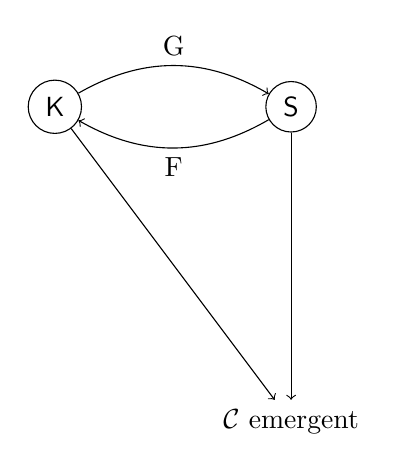
\begin{tikzpicture}[node distance=3cm, auto]
  \node (K) [circle, draw] {$\mathsf{K}$};
  \node (S) [circle, draw, right of=K] {$\mathsf{S}$};
  \draw[->] (K) to[bend left] node {G} (S);
  \draw[->] (S) to[bend left] node {F} (K);
  \node (C) [below of=S, yshift=-1cm] {$\mathcal{C}$ emergent};
  \draw[->] (K) -- (C);
  \draw[->] (S) -- (C);
\end{tikzpicture}
\caption{Mutual generation of SSZK and KSZS gives rise to an emergent category.}
\end{figure}

\section{Discussion and Future Work}
This framework suggests that categorical structures need not be fundamental. Instead, they arise from dual generative principles reminiscent of decoherence/coherence dynamics. Further work will refine these structures, connect them with topos-theoretic ideas, and explore potential applications to quantum foundations.

\section*{Acknowledgments}
A categorical theory on the emergence of truth, dedicated to Nagarjuna for the insight of Sunyata (Emptiness).

\end{document}
